\section{Caesar Cipher}

\subsection{Dari Teori ke Praktik: Modular Arithmetic dalam Aksi}

Dalam Bab III, kita mempelajari aritmetika modular sebagai fondasi matematika kriptografi. Sekarang, kita akan melihat penerapan pertama dan paling sederhana dari konsep ini: \textbf{Caesar Cipher}.

Caesar cipher adalah contoh sempurna bagaimana matematika abstrak menjadi alat praktis:
\begin{itemize}
  \item \textbf{Teori (Bab III)}: $a \equiv b \pmod{n}$, operasi modular
  \item \textbf{Praktik (Bab IV)}: $E_k(x) = (x + k) \bmod 26$
  \item \textbf{Implementasi}: Kode C yang menerapkan operasi ini
\end{itemize}

Ini adalah langkah pertama dari teori ke aplikasi—sebuah pola yang akan terus kita lihat dalam cipher yang lebih kompleks.

\subsection{Konsep}

Caesar cipher adalah cipher substitusi paling sederhana: setiap huruf digeser sejumlah $k$ posisi dalam alfabet (0--25). Enkripsi:
\[
E_k(x) = (x + k) \bmod 26
\]
Dekripsi:
\[
D_k(y) = (y - k) \bmod 26
\]

Huruf A=0, B=1, ..., Z=25. Dengan $k=3$: A$\to$D, B$\to$E, ..., Z$\to$C.

\begin{contoh}
Plaintext: HELLO, $k=3$. H$\to$K, E$\to$H, L$\to$O, L$\to$O, O$\to$R. Ciphertext: KHOOR.
\end{contoh}

Caesar cipher dinamai dari Julius Caesar yang menurut sejarahwan menggunakan cipher ini dengan shift tiga posisi untuk melindungi pesan militer \cite{stallings2017}. Cipher ini membentuk fondasi untuk teknik substitusi dan analisis frekuensi.

\subsection{Koneksi ke Matematika Bab III}

Mari kita lihat bagaimana Caesar cipher langsung menerapkan konsep dari Bab III:

\textbf{1. Aritmetika Modular}: 
\begin{itemize}
  \item Operasi enkripsi: $(x + k) \bmod 26$ menggunakan modular arithmetic
  \item Operasi dekripsi: $(y - k) \bmod 26$ juga modular arithmetic
  \item Modulus 26 karena ada 26 huruf dalam alfabet Inggris
\end{itemize}

\textbf{2. Invers Modular}:
\begin{itemize}
  \item Dekripsi adalah "invers" dari enkripsi
  \item $(x + k - k) \bmod 26 = x \bmod 26$ — dekripsi berhasil
  \item Ini adalah contoh sederhana dari konsep invers yang akan penting dalam cipher lebih kompleks
\end{itemize}

\textbf{3. Representasi $\mathbb{Z}_{26}$}:
\begin{itemize}
  \item Huruf diubah menjadi angka 0-25 (elemen $\mathbb{Z}_{26}$)
  \item Operasi dilakukan dalam $\mathbb{Z}_{26}$
  \item Hasil dikonversi kembali ke huruf
\end{itemize}

Meskipun Caesar cipher sangat lemah oleh standar modern, cipher ini memiliki nilai edukasi yang penting. Ruang kunci hanya 25 membuatnya rentan brute force \cite{schneier1996}. Pemahaman Caesar cipher menjadi langkah pertama untuk memahami cipher substitusi dan kriptanalisis dasar.

\subsection{Pemetaan Huruf dan Ruang Kunci}

Caesar cipher memiliki $25$ kunci efektif (shift 1--25), karena $k=0$ atau $k=26$ menghasilkan teks asli. Pemetaan huruf bisa ditulis sebagai tabel (contoh shift $k=3$) \cite{stallings2017}:
\begin{table}[htbp]
  \centering
  \small
  \begin{tabular}{cccccccccc}
    \toprule
    P & A & B & C & D & E & F & G & H & I \\
    \midrule
    C & D & E & F & G & H & I & J & K & L \\
    \bottomrule
  \end{tabular}
  \caption{Pemetaan sebagian huruf untuk Caesar dengan $k=3$.}
\end{table}

\begin{figure}[htbp]
  \centering
  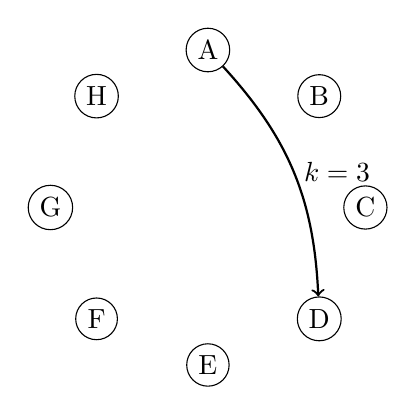
\begin{tikzpicture}[scale=1]
    \foreach \i/\ch in {0/A,1/B,2/C,3/D,4/E,5/F,6/G,7/H} {
      \node[circle, draw, inner sep=2pt] (p\i) at ({90-45*\i}:2) {\ch};
    }
    \draw[->, thick] (p0) to[bend left=20] node[midway, right] {$k=3$} (p3);
  \end{tikzpicture}
  \caption{Ilustrasi pergeseran Caesar (contoh terbatas A--H).}
\end{figure}

Pemetaan huruf sistematis penting untuk implementasi yang efisien. Ruang kunci yang terbatas (25 kemungkinan) membuat Caesar rentan terhadap brute force \cite{trappe2006}.

\subsection{Brute Force dan Analisis Keamanan}

Karena ruang kunci kecil, semua kemungkinan $k$ dapat dicoba. Misal ciphertext KHOOR:
\begin{table}[htbp]
  \centering
  \small
  \begin{tabular}{cc}
    \toprule
    $k$ & Hasil dekripsi \\
    \midrule
    1 & JGNNQ \\
    2 & IFMMP \\
    3 & HELLO \\
    4 & GDKKN \\
    5 & FCJJM \\
    \bottomrule
  \end{tabular}
  \caption{Brute force sederhana untuk Caesar.}
\end{table}

Brute force terhadap Caesar sangat efektif karena ruang kunci kecil \cite{stallings2017}. Demonstrasi brute force berharga untuk memahami mengapa cipher klasik lemah dan mengapa teknik modern diperlukan.

\textbf{Pelajaran untuk Cipher Modern}:
\begin{itemize}
  \item \textbf{Ruang kunci harus besar}: Caesar hanya memiliki 25 kemungkinan
  \item \textbf{Struktur harus kompleks}: Caesar hanya substitusi sederhana
  \item \textbf{Statistik harus tersembunyi}: Caesar mempertahankan frekuensi huruf
\end{itemize}

Ini adalah awal dari perjalanan kita memahami mengapa cipher modern seperti AES dirancang jauh lebih kompleks.

\subsection{Implementasi dalam C}

\begin{lstlisting}[style=cstyle, caption={Caesar Cipher dalam C}]
#include <stdio.h>
#include <ctype.h>
#include <string.h>

void caesar_encrypt(char *text, int shift) {
    int i;
    for (i = 0; text[i] != '\0'; i++) {
        if (isalpha(text[i])) {
            char base = isupper(text[i]) ? 'A' : 'a';
            text[i] = base + (text[i] - base + shift + 26) % 26;
        }
    }
}

void caesar_decrypt(char *text, int shift) {
    caesar_encrypt(text, 26 - shift);
}

int main() {
    char msg[] = "HELLO CRYPTO";
    caesar_encrypt(msg, 3);
    printf("Encrypted: %s\n", msg);   /* KHOOR FUBVWR */
    caesar_decrypt(msg, 3);
    printf("Decrypted: %s\n", msg);   /* HELLO CRYPTO */
    return 0;
}
\end{lstlisting}

Implementasi Caesar cipher dalam C menunjukkan bagaimana konsep matematika sederhana dapat diterjemahkan menjadi kode praktis yang fungsional. Fungsi ini menggunakan pendekatan tabel implisit dengan mengkonversi karakter ke indeks numerik (0-25) sebelum melakukan operasi modular. Implementasi ini juga menangani karakter non-alfabet dengan membiarkannya tidak berubah, yang merupakan praktik baik dalam aplikasi nyata.

\textbf{Koneksi ke Implementasi Lanjutan}:
\begin{itemize}
  \item Pola implementasi ini akan kita lihat lagi dalam cipher yang lebih kompleks
  \item Teknik modular arithmetic akan digunakan dalam Vigenère, Affine, dan Hill cipher
  \item Prinsip enkripsi/dekripsi invers akan menjadi fundamental dalam semua cipher
\end{itemize}

Dalam implementasi produksi, fungsi seperti ini sering dioptimasi dengan menggunakan lookup table untuk pergeseran huruf daripada menghitung operasi modular untuk setiap karakter. Optimasi ini sangat penting untuk aplikasi yang memproses volume teks besar, seperti enkripsi file atau streaming data. Selain itu, implementasi yang robust harus menangani berbagai encoding karakter (ASCII, UTF-8) dan kasus edge seperti input kosong atau karakter tidak valid.
